\documentclass[11pt,twoside]{scrreprt}

\renewcommand{\textfraction}{0.001}
\renewcommand{\topfraction}{0.999}   
\renewcommand{\bottomfraction}{0.999}

\usepackage{graphicx}
\usepackage{amsmath}
\usepackage{mathtools}
\usepackage{amssymb}
\usepackage[bibencoding=utf8, backend=biber, style=numeric, minbibnames=1, maxnames=5]{biblatex}
\addbibresource{bibliography.bib}
\usepackage{a4,color}
\usepackage{tikz}
\usepackage{pgfplots}
\pgfplotsset{compat=1.10}
\usepackage{calc}

\usepackage{booktabs}
\usepackage{caption}
\usepackage{subcaption}
\usepackage{float}
\usepackage{url}
\usepackage{listings}

\usepackage[T1]{fontenc}
\usepackage[utf8]{inputenc}

\usepackage{mathpazo}

\definecolor{red}{rgb}{1,0,0}
\definecolor{green}{rgb}{0,1,0}
\definecolor{blue}{rgb}{0,0,1}
\definecolor{darkblue}{rgb}{0,0,0.8}

\definecolor{yellow}{rgb}{1,1,0}
\definecolor{lightblue}{rgb}{0,1,1}
\definecolor{magenta}{rgb}{1,0,1}
\definecolor{lightgrey}{rgb}{0.5,0.5,0.5}
\definecolor{grey}{rgb}{0.35,0.35,0.35}
\definecolor{darkgrey}{rgb}{0.2,0.2,0.2}
\definecolor{ockerrot}{rgb}{0.859,0.375,0.152}

% Default fixed font does not support bold face
\DeclareFixedFont{\ttb}{T1}{txtt}{bx}{n}{12} % for bold
\DeclareFixedFont{\ttm}{T1}{txtt}{m}{n}{12}  % for normal

% Custom colors
\usepackage{color}
\definecolor{deepblue}{rgb}{0,0,0.5}
\definecolor{deepred}{rgb}{0.6,0,0}
\definecolor{deepgreen}{rgb}{0,0.5,0}

\usepackage{listings}

% Python style for highlighting
\lstset{
language=Python,
basicstyle=\ttm,
otherkeywords={self, for},             % Add keywords here
keywordstyle=\ttb\color{deepblue},
emph={MyClass,__init__, np},          % Custom highlighting
emphstyle=\ttb\color{deepred},    % Custom highlighting style
stringstyle=\color{deepgreen},
frame=tb,                         % Any extra options here
showstringspaces=false            % 
}


\captionsetup{margin=0pt,font=small,labelfont=sc,labelformat=simple,format=plain,indention=3mm,
 labelsep=endash,textfont=sf,font=sf,singlelinecheck=on,figurename=Fig.,tablename=Tab.}


\fontfamily{ppl}\selectfont

\newcommand*{\bfrac}[2]{\genfrac{\big (}{\big )}{0pt}{}{#1}{#2}}

\setlength{\parskip}{1.5ex plus 0.5ex minus 0.2ex}
\setlength{\parindent}{0pt}

\begin{document}

\chapter*{Abstract}
\addcontentsline{toc}{chapter}{Abstract}
This thesis studies an algorithms for the detection of circles which are produced by particles travelling through the RICH detectors generating Cherenkov radiation.
At the beginning there is an introduction to the linear hough transform and then to the hough transform to detect circles. The first case considered
is when there is only one unknown (radius) and the center is known. The second case is with two unknowns where the radius is known but the center unknown ($(x,y)$
coordinates of the center are the two unknown parameters).
Lastly there is the case where all the parameters are unkown. For this case there is on the one hand the traditional approach studied with the conventional accumulator
space and on the other hand a new approach is developped and studied. This approach works on the basis that each circle is defined by 3 points. Once there are three
points the radius and the center can be caculated.

\tableofcontents
\listoftables
\listoffigures	

\chapter{Introduction}
\section{LHC - Large Hadron Collider} % (fold)
\label{sec:lhc_large_hadron_collider}
\begin{figure}[b]
  \centering
  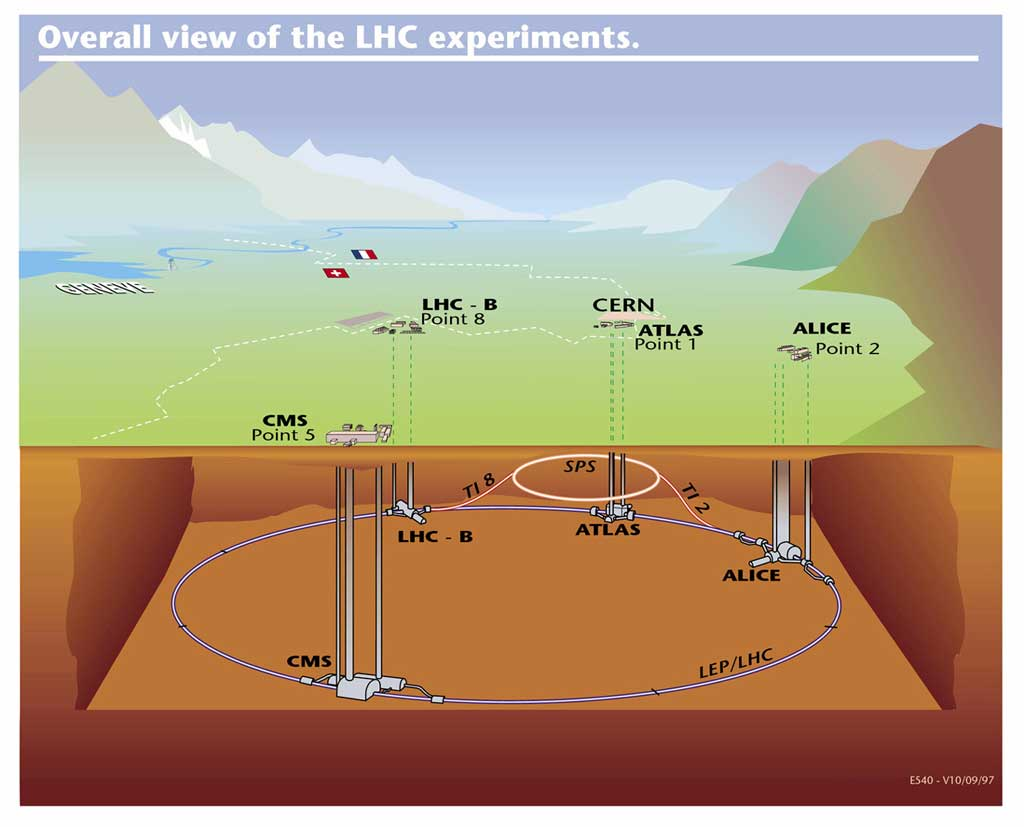
\includegraphics[width=0.6\textwidth]{pics/lhc}
  \caption{The LHC ring with its 4 experiments: ATLAS, CMS, Alice and LHCb}
  \label{fig:lhc}
\end{figure}

The Large Hadron Collider (LHC) is a proton-proton collider. It is the largest and highest-energy particle accelerator in the world. It was built by the European Organisation for Nuclear Research from 1998 to 2008. It aims to test the predictions of different theories in high-energy particle physics, and in particular for the search of the Higgs boson (which has been confirmed this year) and signs for new physics beyong the Standard Model of particle physics. The LHC lies in a tunnel 27\,km in circumference and 100\,m below the surface of the French-Swiss border near Geneva. The LHC was built in collaboration with over 10000 scientists and engineers from over 100 countries. The accelerator has been running with a center of mass energy $\sqrt{s} = 13$ TeV since 20 May 2015.


The core physics programm for the period 2014-2015 includes:

\begin{itemize}
  \item <COMMENT: PROGRAM>
\end{itemize}



% section lhc_large_hadron_collider (end)

\section{LHCb}

\begin{figure}[tb]
  \centering
  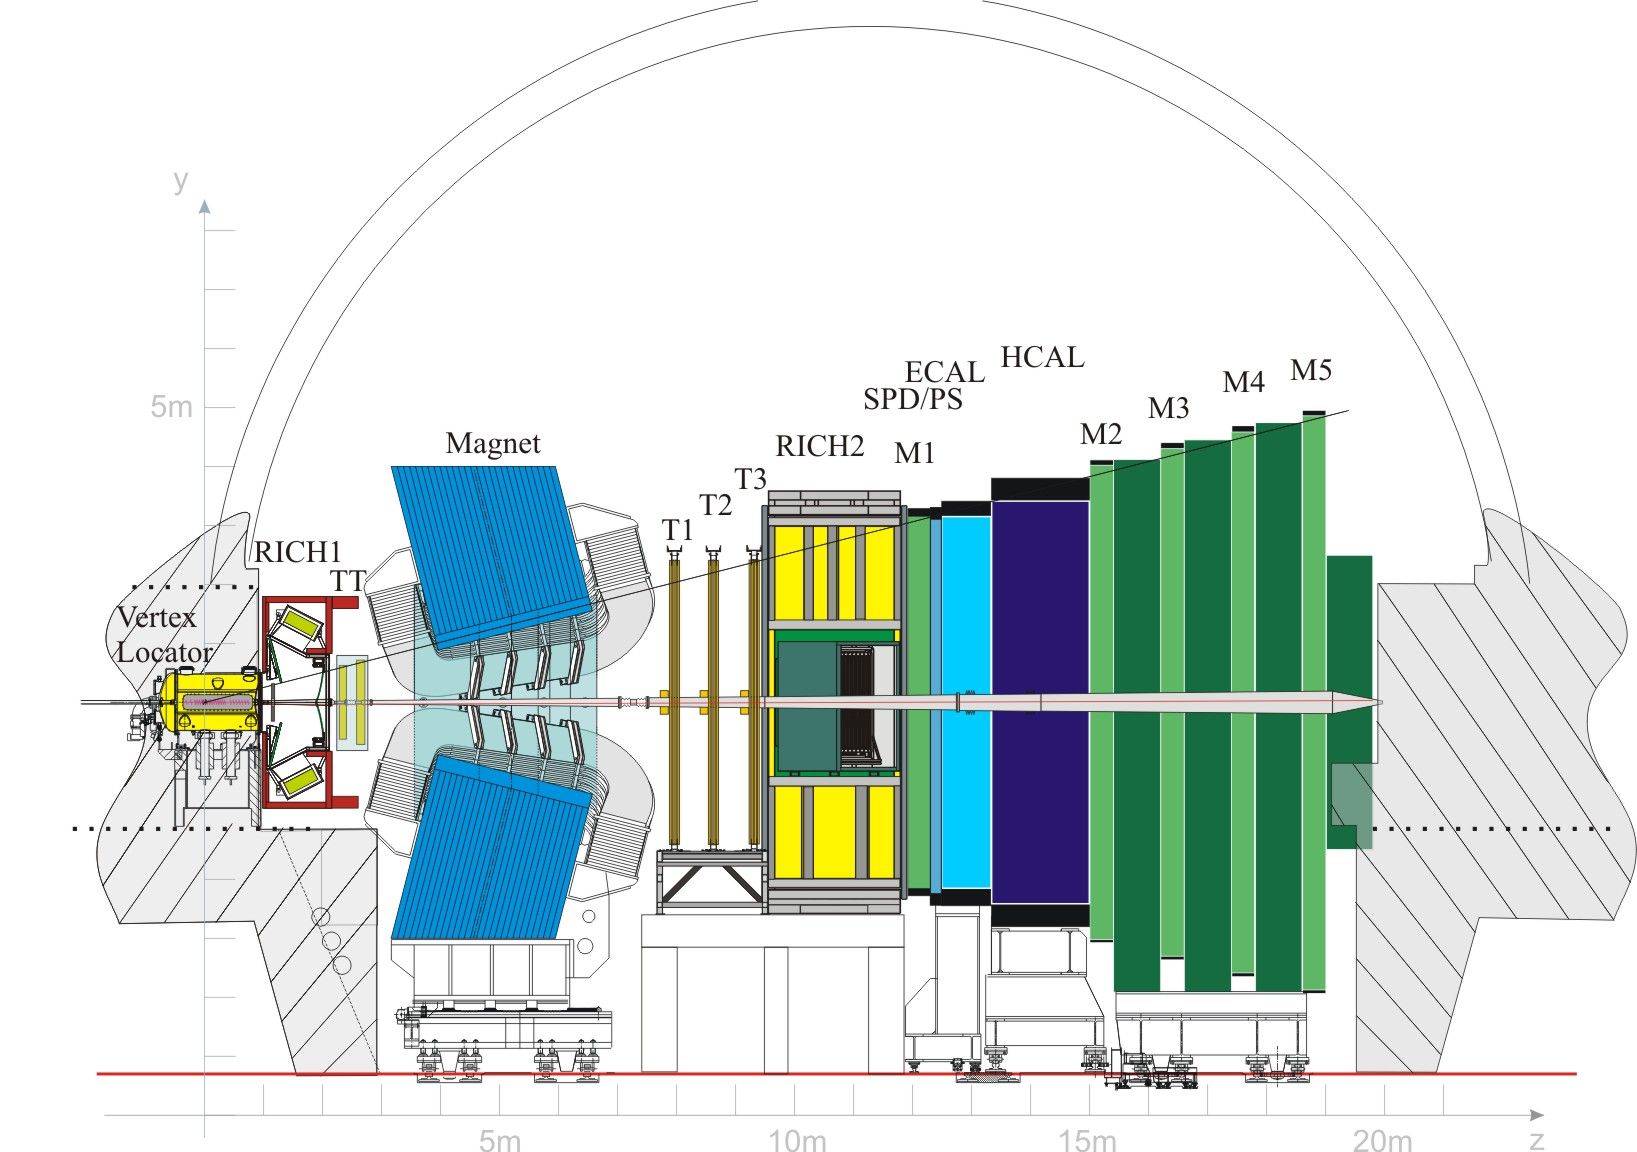
\includegraphics[width=\textwidth]{pics/lhcb_detector}
  \caption{LHCb Detector: RICH1 before the magnet and RICH2 after the magnet with silicon strip detector in between and muon and calorimeter at the end.}
  \label{fig:lhcb}
\end{figure}

The LHCb is one of the four big experiments conducted at the LHC (ATLAS, CMS and ALICE being the other 3). The aim of this experiment is the study of decays of particles containing $b$ and $\bar{b}$ particles (B-Mesons). During collisions these particles don't fly in all direction but rather stay close to the beam pipe. This is reflected in the design of the LHCb detector which is a foward arm spectrometer 20 meters long with subdetectors along the beam pipe as seen in figure \ref{fig:lhcb}.

A quick overview of the detector parts \parencite{lhcbweb}.

\paragraph{VELO} The VErtex LOcator is where the beams collide and $b$/$\bar{b}$ are produced. The VELO measures the distance between the photon collision point and the point where B particles decay. Thus the B particles are not measured directly but inferred from the separation of these two points.

\paragraph{RICH} The RICH detectors are bult for particle identification. One detector on each side of the magnet are used to cover different momentum ranges. RICH detectors work by measuring emissions of Cherenkov radiation which is emmited if a particle travels faster than the speed of light through a certain medium (often compared to breaking the sound barrier).

\paragraph{Magnet} A particle normally moves in a straight line but entering a magnetic field causes the path of charged particles to curve according to the Lorentz force \[
  \mathbf{F} = q\left( \mathbf{E} + \left( v\times\mathbf{B}\right)\right)
\]
thus allowing to determine the charge of the particle. Also the track curvature can be used to infer the momentum of the particle.

\paragraph{Tracking System} The tracking system is based on 4 large tracking stations, each covering about $40$\,m$^2$. It is used to determine the position where the particle passed the detector. In the silicon detector a charge gets deposited on a strip which defines the position and in the gas-filled tubes of the outer tracker a passing particle ionizes the gas molecules producing electrons.

\paragraph{Calorimeters} They are designed to stop particles and measing the amount of energy lost while coming to a halt. The design of the stations is sandwich like. One metal plate and one plastic plate. A particle hitting the metal plate causes a secondary shower which induces a UV light in the plastic plate. The energy lost is proportional to the amount of light emmitted. It is the main way of identifying particles with no charge (e.g. photons, neutrons).

\paragraph{Muon system}
Muons are present in the final stage of B decays and thus important for the LHCb experiment. There are 5 rectangular stations increasing in size at the end of the detector. The total area covered by these stations is about $435$\,m$^2$. Each station is filled with a combination of 3 gases. Passing muons react with this mixture and wire electrodes detect the result.
% The fact that at the LHC b-hadrons are predominantly produced in the forward region was used in the construction of the detector. The \emph{LHCb} experiment is a single arm forward spectrometer with a 4\,Tm dipole magnet and a polar angular coverage from 10 to 300 mrad in the horizontal plane (the bending plane of the dipole magnet) and 250 mrad in the vertical plane.


\subsection{Particle Identification} % (fold)
\label{sub:particle_identification}
An important requirement at LHCb is the particle identification. This is handled by CALO, Muon and RICH sub-detectors. The Calorimeters beside measuring energies and positions of electrons, photons and hadrons also provide indentification of said particles. The Muon system identifies muons to a very high level of purity which is esential for many \(J/\Psi\)'s in their final states.

Hadron identification is very important for decays where the final states of interest are purey hadronic. The LHCb RICH system provides. It is composed of two detectors. One positioned upstream of the dipole magnet and the other one positioned downstream of the dipole magnet. The optics is arranged similarly in both sub-detectors: spherical focusing mirrors project the Cherenkov photons onto a series of flag mirrors which then reflect them onto a series of photon detector arrays, located outisde the detector acceptance~\cite{Powell:2011}.



% subsection particle_identification (end)

\chapter{Theory}

\section{Cherenkov-Radiation} % (fold)
\label{sec:cherenkov_radiation}

The speed of light in vacuum, \( \mathbf{c} \), is a universal physical constant. According to Einstein's special theory of relativity, \( c \) is the maximum speed at which all matter (or information) in the universe can travel. The speed at which light propagates in a medium, however, can be significantly less can \( c \).

Cherenkov radiation results when a charged particle travels through a dielectric medium with a speed greather than the speed of light through said medium. Moreover, the velocity that must be exceeded is the phase velocity (\( v_{\text{Phase}} \text{ or short } v_{\text{P}} \)) and not the group velocity \( v_{\text{Group}} = \frac{\partial \omega}{\partial k} \).

\[ v_{\text{P}} = \frac{\lambda}{T} \quad \text{or} \quad \frac{\omega}{k}\]

As a charged particle travels through the medium, it disrupts the local electromagnetic field. If the particle travels slowly then the disturbance elastically relaxes to the mechinal equilibrium as the particle passes. However, if the particle travels fast enough, the limited response speed of the medium means that a disturbance is left in the wake of the particle, and the energy in this disturbance radiates as coherent shockwave.

\begin{figure}[htbp]
  \centering
    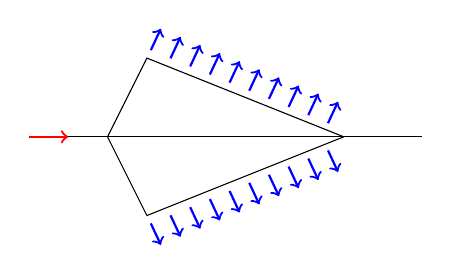
\begin{tikzpicture}
      \draw (-1,0) -- (4,0);
      \draw (0,0) -- (0.5,1) -- (3,0);
      \draw (0,0) -- (0.5,-1) -- (3,0);
      \draw[->, red, thick] (-1,0) -- (-0.5,0);
      \foreach \x in {0,1,...,9} {
        \draw[->,blue, thick] (0.55 + \x*0.25, 1.1 - \x*0.103)  --+ (65:0.3);
        \draw[->,blue, thick] (0.55 + \x*0.25, -1.1 + \x*0.103) --+ (-65:0.3);
      }
    \end{tikzpicture}
  \caption{Cherenkov radiation}
  \label{fig:label}
\end{figure}

\begin{align}
    x_p &= v_{p}\cdot t = \beta c t \nonumber \\
    x_{\text{em}} &= v_{\text{em}}\cdot t=\frac{c}{n}t \nonumber \\
    \cos\theta &= \frac{x_{\text{p}}}{x_{\text{em}}} = \frac{\frac{c}{n}t}{\beta c t} = \frac{1}{n\beta} \nonumber
\end{align}
which is independent from the angle \( \theta \).

\section{RICH Detector} % (fold)
\label{sec:rich_detector}

Particle identification is a fundamental requirement at the LHCb experiment. Meaningful CP-violation measurements are only possible if hadron identification is available hence the ability to distinguish between kaons and pions is  essential.
The LHCb experiment is unique in the sense that its hadronic particle identification is handled only by the RICH sub-detectors. This means -- as mentioned before -- that the RICH has to cover a wide range of momentum (1-100 $\text{GeV}/c$).

The RICH-1 in front of the magnet covers a lower momentum range from 1-60 $\text{GeV}/c$. It is composed of 5\,cm thick aerogel tiles arranged around the beam pipe. The aerogel with $n=1.03$ is suited for the lowest momentum tracks. Directly behind the aerogel is circa 1\,m of $\text{C}_4\text{F}_{10}$ which covers the intermediate region of momentum.
For the highest momentum tracks, gaseous $\text{C}\text{F}_4$ is used in the RICH-2.

There is a strong corelation between the polar angle and momentum of the tracks. Tracks with a wider angle often have lower momentum. That is why RICH-1 with the aerogel is located before the dipole magnet so tracks with low momentum will be covered before they swept out of the acceptenace by the magnet.

Both sub-detectors are located in low magnetic field regions to keep the tracks straight while they pass through the radiators.

\begin{figure}[tb]
  \centering
  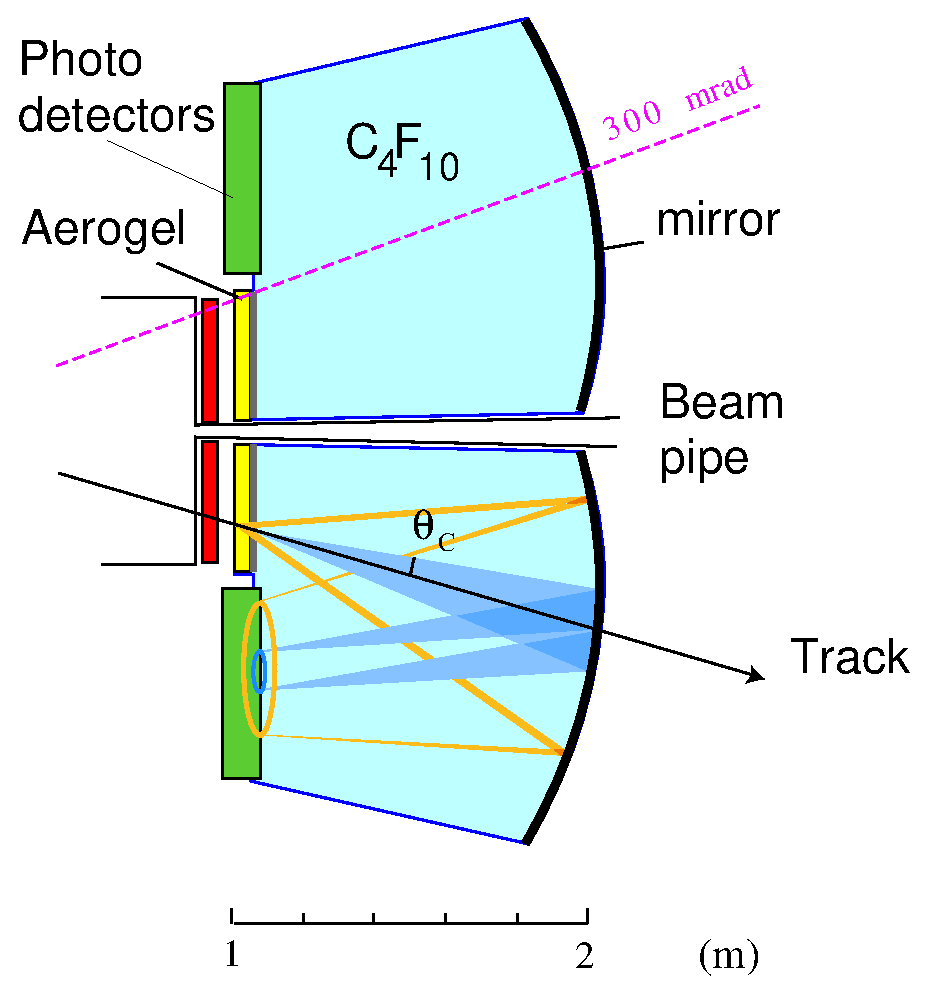
\includegraphics[width=0.5\textwidth]{pics/rich1_schematic}
  \caption{RICH-1 detector \cite{LHCb:2000}.}
  \label{fig:rich1}
\end{figure}
% section rich_detector (end)


% section cherenkov_radiation (end)

\section{Hough Transform} % (fold)
\label{sec:hough_transform}

The Hough-Transform is a feature extraction technique used in image analysis, computer vision and digital image processing.

the purpose is to find imperfect instances of objects within a certain cass of shapes by a voting procedure. This voting procedure is carried out in a parameter space from which object candidates are obtained as local maxima in a so called accumlator space that is explicitly constructed by the algorithm for computing the Hough-Transform.

Initially the Hough-Transform was concerned with finding straight lines but has been extended to identifying positions of arbitrary shapes, such as circles and ellipses.

\subsection{Linear Hough Transform} % (fold)
\label{sub:linear_hough_transform}

A linear function is normally defined as the following:

\[
  f(x) = m\cdot x + b
\]
where $m$ is the slope of the line and $b$ the intercept. For the Hough-Transform however, this representation is not ideal. For a vertical line $m$ would go to infinity which gives us an unbound transform space for $m$. For this reason Duda and Hart suggested the $\rho\text{-}\theta$ parametrization \parencite{Duda:1972}.

\[
  r = x\cos\theta + y\sin\theta
\]
where $r$ is the distance from the origin to the closest point in the line and $\theta$ is the angle between the $x$-axis and the line connecting the origin with that closest point.

\begin{figure}[ht]
  \centering
  \begin{tikzpicture}[scale=3]
    \draw[<->] (0,1.5) -- (0,0) -- (1.5,0);
    \draw[red,semithick] (0,1) -- (1,0);
    \draw[blue, -> ,semithick] (0,0) -- (0.5, 0.5);
    \draw[semithick,blue] (0.2,0) arc (0:45:0.2cm);
    \node[below] at (0.1,0.121) {\footnotesize$\rho$};
    \node[above] at (0.2,0.2) {$r$};
  \end{tikzpicture}
  \caption{$\rho\text{-}\theta$ parametrisation}
  \label{fig:rhotheta}
\end{figure}
% subsection linear_hough_transform (end)

This means given a single point in the plane, the set of all lines going through this point form a sinusoidal curve in $\rho\text{-}\theta$ space. Another point 
that lies on the same straight line in the plane will produce a sinusoidal curve that intersects with the other at ($\rho\text{-}\theta$) and so do all the points lying on the same straight line. 

\subsubsection{Example of a Linear HT} % (fold)
\label{ssub:example_of_a_linear_ht}
  
\begin{tikzpicture}
  \draw[<->] (3,0) -- (0,0) -- (0,3);

  \foreach \x in {0,0.5,1} {
    \draw[fill] (2-\x, 2-\x) circle (1pt);
  }

  \draw[red] (-0.1,-0.1) -- (2.2,2.2);
\end{tikzpicture}
\begin{table}
\centering
\caption{Angle vs Distance}
\begin{tabular}{rr}
\toprule
 Angle & Distance \\
\midrule
0 & 2.334 \\
\bottomrule
\end{tabular}
\end{table}

% subsubsection example_of_a_linear_ht (end)


\subsection{Circle Hough Transform} % (fold)
\label{sub:circle_hough_transform}

For this thesis we are interested in circle detection so we need to adapt our linear Hough Transform in order to find circles. In a two dimensional space, a circle can be described by:

\begin{equation}
		(x-c_x)^2 + (y-c_y)^2 = r^2
\end{equation}

Where $(c_x,c_y)$ is the center of the circle and $r$ the radius. The possible parameters for the parameters space are now $c_x, c_y$ and $r$. This means if we know the center of the circle the parameter space is one-dimensional and if we know the radius of the circle our parameter space is two-dimensional and of course if we know nothing the parameter space is three-dimensional.



% subsection circle_hough_transform (end)
% section hough_transform (end)


\chapter{Methods}

\section{Conventional Hough-Transforms} % (fold)
\label{sec:conventional_hough_transforms}

In the following subsections we discuss the conventional Hough-Transforms for the case of a one, two and three dimensional parameter space. These
methods were mainly considered to get an idea what was possible with the conventional hough transform. For closer study the method of choice was
the combinatorial approach discussed in depth in section \ref{sec:combinatorial_approach}.
% section conventional_hough_transforms (end)

\subsection{1D: Known Center - Find Radius} % (fold)
\label{sub:1d_known_center_find_radius}

In this case the center(s) of the circle(s) is/are known so only the radius is missing. For the radius there is an array with a minimum value
and increasing by a defined stepsize to the maximum possible radius value. For the example in this thesis the minimum is $0$, the maximum radius
is $1$ and stepsize equal to $0.001$. Introducing following scoring function $\eta(r)$ allows to find the right radius.

\begin{equation}
\label{eq:score_function}
  \eta(r) = (c_x - x)^2 + (c_y - y) - r ^ 2
\end{equation}

and using this in a gauss distribution

\begin{equation}
\label{eq:weight_function}
  w(\eta) = \frac{1}{\sqrt{2\pi}\sigma}\exp\left( \frac{-\eta^2}{2\sigma^2}\right)
\end{equation}
\begin{figure}[tb]
  \centering
  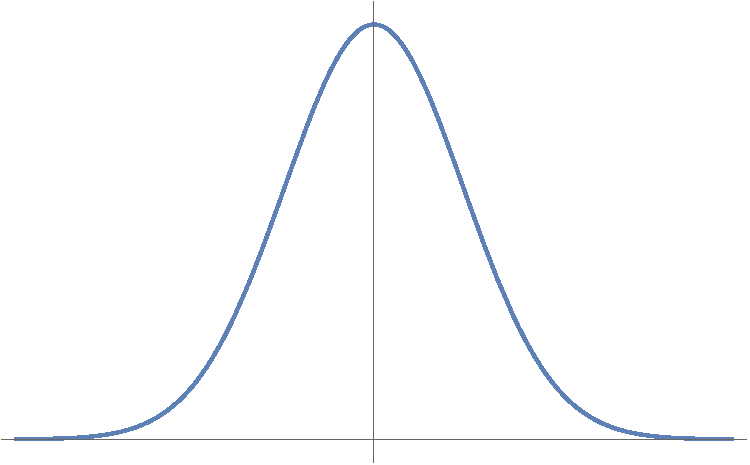
\includegraphics[width=0.5\textwidth]{pics/gauss}
  \caption{Using the probability density function of the normal distribution to calculate the score of a point in order to have a well defined maximum if a point
  lies directly on the circle and $\eta(r) = 0$. }
  \label{fig:gauss}
\end{figure}
This is of course just the circle equation with $c_x, c_y$ being the center of the circle, $x, y$ are the data points and $r$ the radius.
So if a lot of the data points have the same distance $r$ from the circle center there will be a high score for this particular radius. The index
forthe highest score can then be used to find the corresponding radius.

\begin{figure}
  \begin{lstlisting}
  DMENSION = 1001
  r= linspace(0,1,DIMENSION)
  for c in centers:
    scores = zeros(DIMENSION)
    for x,y in allPoints:
      s = 2*BIN_WIDTH
      eta = (c_x-x)**2 + (c_y-y)**2 - r**2
      scores += 1. / ( sqrt( 2 * Pi ) * s ) 
                 * exp( -( eta ** 2 ) 
                  / ( 2 * s ** 2 ) )
  
    index = max(scores)
    circle = {}
    circle['center'] = c
    circle['radius'] = r[index]
\end{lstlisting}
\caption{Pseudo code for the 1D Hough Transform. r is an array of length 1001 so $\eta$ will also be an array of length 1001. Scores is where the score for each iteration is stored. For each point the score is computed and added to the scores array and at the end the index with the highest score is the index we need to get the radius.}
\end{figure}

\subsubsection{Runtime} % (fold)
The runtime of this algorithm is of $\mathcal{O}(n)$ where $n$ is the dimension of the radius array.
\label{ssub:runtime_1d}

% subsubsection runtime (end)

% subsection 1d_known_center_find_radius (end)
\subsection{2D: Known Radius - Find Center} % (fold)
\label{sub:2d_known_radius_find_center}
Now the radius is known and the $x$ and $y$ coordinate of the center $(c_x, c_y)$ are unknown. Now instead of a one dimension the accumulator is 2 dimensional. The range of that space is simply the dimension of the plane which for this thesis is generally $[-0.5,0.5]$. Size of the bins is 0.001. So if the plane was 1 m wide the accuracy of the accumulator is up to 1 mm. As in the one dimensional case we use the scoring function \ref{eq:score_function} in combination with the weight function \ref{eq:weight_function}.

\begin{figure}[b]
\begin{lstlisting}
  DIMENSION = 1001
  xbins = linspace(-0.5,0.5,DIMENSION)
  ybins = linspace(-0.5,0.5,DIMENSION)
  x, y = broadcast_arrays( xbins[..., newaxis], 
                           ybins[newaxis,...] )

  for r in Radiuses:
    weights = zeros( (DIMENSION,DIMENSION) )
    for xd,yd in allPoints:
      s = 2*BIN_WIDTH
      eta = (xd-x)**2 + (yd-y)**2 - r**2      
      weights += 1. / ( sqrt( 2 * pi ) * s ) 
                 * exp( -( eta ** 2 ) 
                 / ( 2 * s ** 2 ) )
    i, j = argmax(weights)
    removeUsedPoints()
    circle['Center'] = (xbins[i], ybins[j])
    circle['Radius'] = r
\end{lstlisting}
  \caption{Pseudo code for the 2D Hough Transform. xbins and ybins are arrays of length 1001. Here we use array broadcasting in order to avoid for loops and the weights can be evaluated in one line. This means that the x and y variables have dimension (1001,1001) but they don't take up that much memory. The x variable for example just broadcasts its value from the first row down to all the other rows and for y it broadcasts the first column to all the other columns. Weights variable is a 1001 by 1001 matrix. Again the entry with the highest score is the candidate for a possible circle center and if found stores in a final variable called circle.}
\end{figure}


\subsubsection{Runtime} % (fold)
\label{ssub:runtime_2d}
The runtime of this algorithm is $\mathcal{O}(n^2)$ where $n$ is the dimension of the histogram. The calculation of the weight has to be done for each data point of the 2D histogram. So in a $1000\times 1000$ histogram with 400 data points we calculate 400'000'000 times the weight of a grid point. Reducing the dimensions of the histogram weakens the accuracy of the whole algorithm but can speed up the calculations considerably. With a $1000\times 1000$ histogram the resolution in each space dimension is $1$\,mm. The RICH Technical Design Report states the resolution of the HPD is $2.5$\,mm $\times$ $2.5$\,mm.

The need (not entirely true) to calculate the weight for each grid point and data point means that there is a loop over data points and two loops for the $x$ and $y$ coordinate of the grid. To improve upon that there is the possibility of array broadcasting.
% subsubsection runtime (end)

\subsubsection{Array broadcasting}
Consider following one dimensional arrays where $x$ is a 1D histogram binning entries from 1 to 4 and same for $y$. 
\begin{align*}
  x &= [1, 2, 3, 4]\\
  y &= [1, 2, 3, 4]  
\end{align*}
Now all combinations between an element of $x$ and $y$ represent a 2D grid $\left((1,1), (1,2), ...\right)$. So to iterate through all those grid points one would have to create 2 for-loops iterating through $x$ and $y$

\noindent\begin{minipage}{\linewidth}
\begin{lstlisting}
def funcB():
  a = np.random.randn(100)
  b = np.random.randn(100) 
  for x in a:
    for y in b:
      print (1-x)^2 + (2-y)^2 - 9
\end{lstlisting}  
\end{minipage}
%
This is not only slow but also doesn't look too nice if there are even more loops.
Broadcasting now turns this one dimensional array of length $n$ into an $n\text{ by }n$ matrix
\[
  x = \begin{bmatrix}
  1 & 1 & 1 & 1 \\
  2 & 2 & 2 & 2 \\
  3 & 3 & 3 & 3\\
  4 & 4 & 4 & 4
  \end{bmatrix}
\]
and
\[
  y = \begin{bmatrix}
  1 & 2 & 3 & 4 \\
  1 & 2 & 3 & 4 \\
  1 & 2 & 3 & 4 \\
  1 & 2 & 3 & 4 
\end{bmatrix}
\]
\noindent\begin{minipage}{\linewidth}
And with this the loops can be omitted:
\begin{lstlisting}
def funcA():
  a = np.random.randn(100)
  b = np.random.randn(100) 
  x,y = np.broadcast_arrays(a[...,np.newaxis],
                            b[np.newaxis,...])
  print (1-x)^2 + (2-y)^2 - 9
\end{lstlisting}  
\end{minipage}
In this case this prints a $4$ by $4$ array with the function evualted for each combination of entries of $x$ and $y$
\[
  \begin{bmatrix}
    -8& -9& -8& -5\\
    -7& -8& -7& -4\\
    -4& -5& -4& -1\\
     1&  0&  1&  4
       \end{bmatrix}
\]
%
\begin{minipage}{\linewidth}
A runtime comparison shows   
\begin{lstlisting}
In [3]: %timeit funcA()
10000 loops, best of 3: 76.8 us per loop

In [4]: %timeit funcB()
100 loops, best of 3: 7.99 ms per loop
\end{lstlisting}
So the version with broadcasting is 100 times than the double loop. And the memory consumption is moderate since they broadcasted entries aren't new memory locations but just refer to the initial array.
\end{minipage}


\subsubsection{Optimizations} % (fold)
\label{ssub:optimizations}
It was mentioned before that for each data point the weight for the whole grid has to be calculated, that is not true. In the 2D case each grid point is a potential center for a circle only if it is not further a away and a threshold radius $R_T$, so if a grid point is further away than this threshold radius this calculation could be skipped. This could probably be done even smarter with the use of some sub grid so only points in the surrounding sub grids.

% subsubsection optimizations (end)

\subsection{Simple Example of 2 Circles Without Background} % (fold)
\label{ssub:simple_example_of_2_circles_without_background}
\begin{figure}[hp]
  \centering
  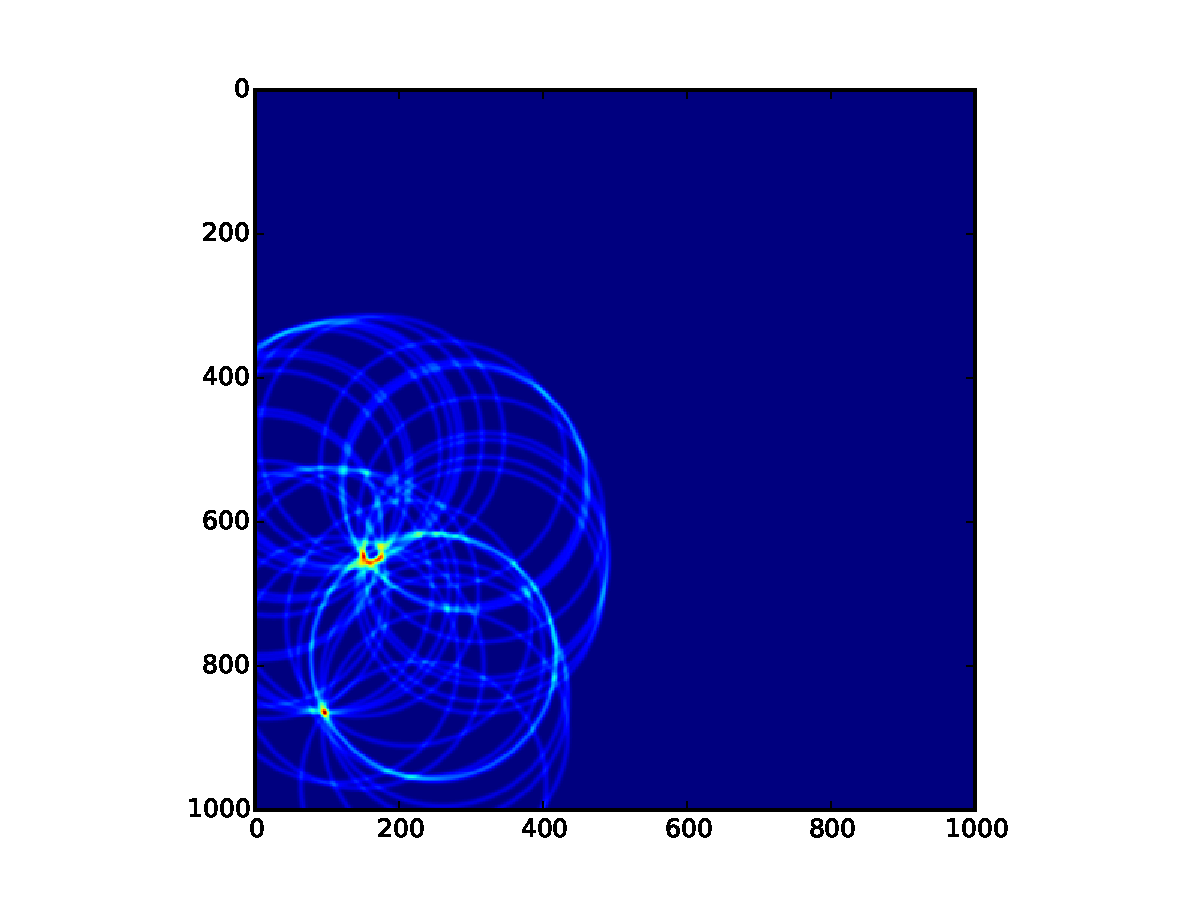
\includegraphics[width=0.8\linewidth]{pics/2d_weights_01}
  \caption{2D weight matrix in the first iteration of the Hough Transform algorithm. The circles have similar radiuses (0.170 and 0.158) which explains one clear maximum in the bottom left and a smeared one a bit to the top right.}
  \label{fig:2d_weights_01}
\end{figure}

\begin{figure}[hp]
  \centering
  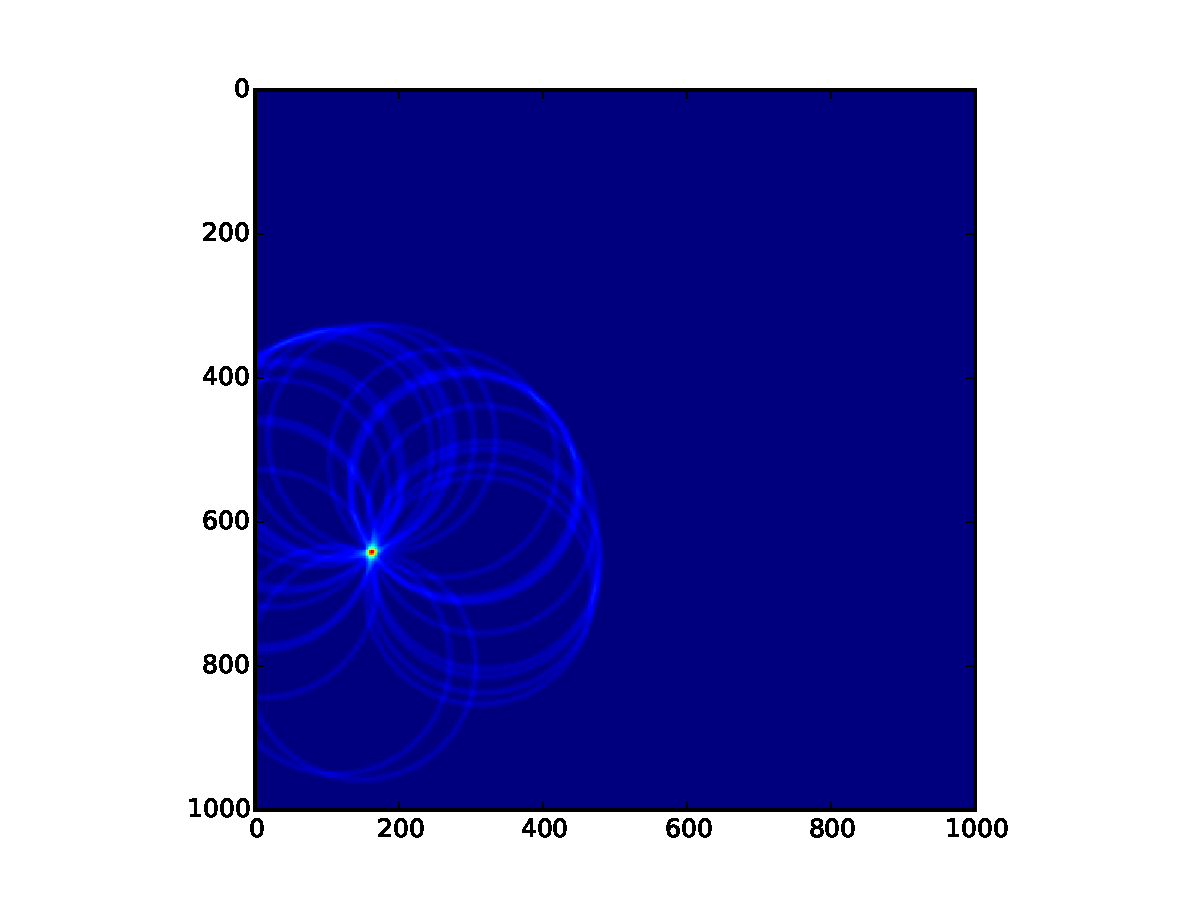
\includegraphics[width=0.8\linewidth]{pics/2d_weights_02}
  \caption{2D weight matrix in the second iteration. Points that satisfied the condition being less than a certain $\epsilon$ away from the radius found in the first iteration are removed leaving (hopefully) only points available that belong to the second circles.}
  \label{fig:2d_weights_02}
\end{figure}
% subsubsection simple_example_of_2_circles_without_noise (end)
% section 2d_known_radius_find_center (end)
\clearpage
\subsection{3D: Nothing is Known - Find Everything} % (fold)
\label{sub:3d_nothing_is_known_find_everything}
In this section all that is known are the data points and the algorithm has to retrieve both center and radius of the circles. The accumulator space
is now in three dimensions. Two for the center coordinate and one for the radius. Similar as to the 2D case array broadcasting is used again
to speed up the calculations of the weight. Furthermore it is the first time that the algorithm has to decide itself whether or not all circles have
been found since there unlike in the previous two cases there isn't any information availabe about the circles so a condition has to be set
to decide when there are no more circles.
\begin{lstlisting}
xbins = np.linspace(-0.5,0.5,DIMENSION)
ybins = np.linspace(-0.5,0.5,DIMENSION)
rbins = np.linspace(0,0.5, R_DIMENSION)

x,y,r = np.broadcast_arrays(\
            xbins[np.newaxis,...,np.newaxis],\
            ybins[np.newaxis,np.newaxis,...],\
            rbins[...,np.newaxis,np.newaxis])
\end{lstlisting}
Broadcasting the $x,y,r$ arrays to speed up the calculations. To display the $x,y$ plane for a fixed radius it is important that rbins is
broadcast along the 2nd and 3rd axis. 
\begin{lstlisting}
while True:
  weights = np.zeros(\
         (R_DIMENSION, DIMENSION, DIMENSION))

  for x0,y0 in data['allPoints']:
    s = 0.001
    eta = (x-x0)**2 + (y-y0)**2 - r**2
    weights += 1./( sqrt( 2 * sconst.pi ) * s )*\
                      np.exp( -( eta ** 2 ) / \
                      ( 2 * s ** 2 ) )
  index = np.argmax( weights )
  rr,ii,jj = np.unravel_index( index, 
              (R_DIMENSION, DIMENSION, DIMENSION))
  score = weights[rr][ii][jj]
  if score < 2100:
    break  
\end{lstlisting}
As before a scoring function is used but this time the scoring function is of the form $f(x,y,r)$ and each point in weights then stands for the score of the
$x,y,r$ entries and their respective value.

Since there is now no information about any of the circles it is unknown how many circles there are so a condition is needed to stop looking for circles.
This algorithm uses a simple score threshold that whenever the highest score
of the weight matrix is less than a defined threshold the algorithm stops
and it is assumed that all circles have been found.
\begin{lstlisting}
circle['center'] = (xbins[ii], ybins[jj])
circle['radius'] = rbins[rr]
circles.append(circle)

used_xy += [tup for tup in data['allPoints'] if
    abs( ( tup[0] - circle['center'][0] ) ** 2 +
         ( tup[1] - circle['center'][1] ) ** 2 -
         circle['radius'] ** 2 ) < 2 * 0.001]
data['allPoints'][:] = 
            [tup for tup in data['allPoints'] if 
    abs( ( tup[0] - circle['center'][0] ) ** 2 + 
         ( tup[1] - circle['center'][1] ) ** 2 - 
         circle['radius'] ** 2 ) >= 2 * 0.001]  
\end{lstlisting}
Finally with the indices found the center and radius are retrieved
from the respective bins and saved to a circle dictionary. In order to
avoid finding the same circle twice or use data points twice a check
is being done to see whether a data point fulfills the requirement
of being a circle point. If that's the case that point will be put
into another list of already used points and the algorithm will not 
use this point anymore.
\subsubsection{Runtime} % (fold)
\label{ssub:runtime}
Assuming that the radius array has the same length as the two space
dimensions means that the complexity of this algorithm is of order 
$\mathcal{O}(N^3)$. As the 1D and 2D Hough Transform the accuracy
directly depends on the binning. Same as for the 2D Hough Transform
too match the resolution of the HPD of the RICH detector a binning of 400 makes sense if the detector dimensions are $1$\,m$\times1$\,m.
% subsubsection runtime (end)

\subsubsection{Optimisations} % (fold)
\label{ssub:optimisations}
As for the 2D HT introducing some kind of sub grid for the $x,y$ 
plane so only grid points in the vicinity of a data point are used
for calculating the score.
% subsubsection optimisations (end)
% subsection 3d_nothing_is_known_find_everything (end)

\section{Combinatorial approach}
\label{sec:combinatorial_approach}
A circle is uniquely defined by 3 points and radius and center can be calculated. If there are 15 points lying on the same circle there are 455 possible combinations of triplets According to the binomial distribution.
\[
   \binom{N}{3} = \frac{N!}{k!(N-k)!}
 \] 
Calculating the center and radius for these 455 triplets should result in the same center and same radius for all the triplets (floating point inaccuracy not considered). 

Having one background hit in addition to the 15 circle hits increases the triplet number to 560. The triplets with points solely consisting of points on the circle still have the same center and radius but the new combinations that now include a background hit will vary and it is unlikely that any two triplets that include the background point will have the same center and radius. Here is an overview of the algorithm used for this thesis.

\begin{enumerate}
\item Build all possible triples of points given the data points
\item For all the point triples calculate the center and the radius of the potential circle
\item Due to constraints in the radius many of the circles with a radius bigger than a certain threshold will be dropped.
\item Create a histogram with the radius distribution. Peaks in the radius distribution hint to a circle.
\item Scan the radius histogram for peaks and look at the center point histogram for the given radius of a peak. If there is also a peak in the center point histogram
      the set of the points of the triples lie on a circle with a radius and center given by the histogram peaks.
\end{enumerate}

\subsection{Generating the triples} % (fold)
\label{sub:generating_the_triples}
For generating the triples the built-in function \texttt{itertools.combinations()} of python is used. The input is an iterable, in our case a
list of tuples (each tuple is the $x$ and $y$ coordinate of a data point) which is used to create all possible combinations of triples (of said tuples).

% subsection generating_the_triples (end)

\subsection{Calculating the Circle given 3 points}

Let $(A,B,C)$ be a triple of points in a 2D plane and $a,b,c$ the length of the sides opposite to the respective corner.
%
The semiperimeter is defined as
%
\begin{equation}
  s = \frac{a+b+c}{2}
\end{equation}
%
using this we can calculate the radius $R$ of the circumcircle of triangle $\overline{ABC}$:
\begin{equation}
  R = \frac{abc}{4\sqrt{s(a+b-s)(a+c-s)(b+c-s)}}
\end{equation}
We have $\lambda_1, \lambda_2, \lambda_3$ as the barycenteric coordinates of the circumcenter:
\begin{align}
  \lambda_1 &= a^2\cdot(b^2+c^2-a^2)\\
  \lambda_2 &= b^2\cdot(a^2+c^2-b^2)\\
  \lambda_3 &= c^2\cdot(a^2+b^2-c^2)
\end{align}
Multiplying a matrix consisting of the column vectors of $A,B,C$ with a column vector of $\lambda_1, \lambda_2, \lambda_3$ and dividing the resulting vector by the sum of the barycentric coordinates (for noramlization) leads to the circumcenter of the triangle $\overline{ABC}$ 
%
\begin{equation}
  \begin{pmatrix}
    A_x & B_x & C_x \\
    A_y & B_y & C_y
  \end{pmatrix} \cdot \begin{pmatrix}
    \lambda_1\\
    \lambda_2\\
    \lambda_3
  \end{pmatrix} = \boldsymbol{P'}
\end{equation}
%
\begin{equation}
  \frac{\boldsymbol{P'}}{\lambda_1+\lambda_2+\lambda_3} = \boldsymbol{P}
\end{equation}
%
\begin{figure}[tb]
\centering
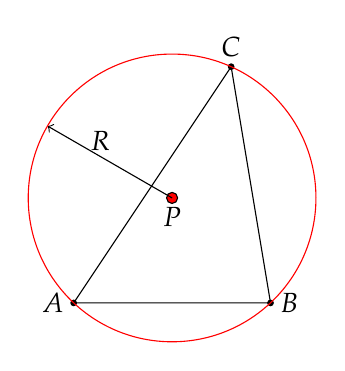
\begin{tikzpicture}
\coordinate (A) at (0,0);
\coordinate (B) at (2.5,0);
\coordinate (C) at (2,3);
\coordinate (Ci) at (1.25,1.33333);
\def\r{1.827}
\draw[thin] (A) -- (B) -- (C) -- cycle;
\node[left] at (A) {$A$};
\node[right] at (B) {$B$};
\node[above] at (C) {$C$};
\node[below] at (0.34,2.3) {$R$};
\draw[fill=black] (A) circle (1pt);
\draw[fill=black] (B) circle (1pt);
\draw[fill=black] (C) circle (1pt);
\draw[fill=red] (Ci) circle (2pt) node [below] (Ci) {$P$};

\draw[->] (1.25,1.33333) -- +(150:1.827);
\draw[red] (1.25,1.33333) circle (1.827);
\end{tikzpicture}
\caption{The circumradius ($R$) and the circumcenter ($P$) of a circle defined by three points.}
\label{fig:circum_fig}
\end{figure}



\subsection{Drawback}
	

There is also a drawback with this method: the combinatorics blow up with a high number of data points \( \binom{N}{3} \). So for example with 200 data points (circle data and background) the number of triplets is

\[ \binom{200}{3} = 1313400 \]
and for 300:
\[ \binom{300}{3} = 4455100 \]

So the runtime of the algorithm is roughly in the order of $\mathcal{O}(N^3)$ which can be easily seen when taking the upper bound of $\binom{N}{k} \leq \frac{N^k}{k!}$ and since $k=3$ then means $\frac{N^3}{3!}$ see figure \ref{fig:binom_growth}. 
\begin{figure}[ht]
\centering
  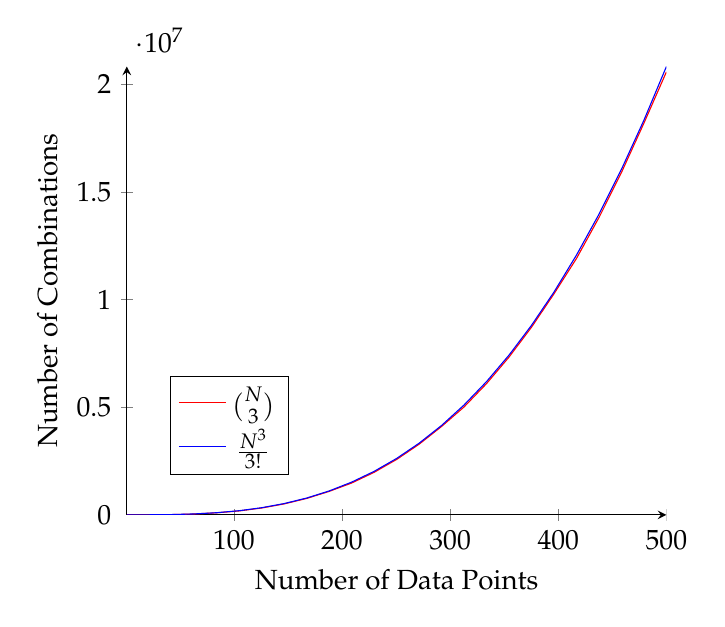
\begin{tikzpicture}
    \begin{axis}[
    axis lines = left,
    xlabel = Number of Data Points,
    ylabel = {Number of Combinations},
    legend style={at={(0.3,0.2)},anchor=east},
    ]
    \addplot [
    domain=1:500, 
    color=red,
    ]
    { factorial(x)/(factorial(x-3)*factorial(3))};
    \addplot [
    domain=1:500, 
    color=blue,
    ]
    { x^3/factorial(3)};
    \addlegendentry{$\binom{N}{3}$}
    \addlegendentry{$\frac{N^3}{3!}$}
    \end{axis}

  \end{tikzpicture}
    \caption{Scaling of the algorithm. Binomial Growth with $\binom{N}{3}$ compared with the approximation $\frac{N^3}{3!}$. So the algorithm runs in the order of $\mathcal{O}(n^3)$}
  \label{fig:binom_growth}
\end{figure}

\subsubsection{Optimisation} % (fold)
\label{ssub:improvement_of_speed}

As seen before this approach scales with $\binom{N}{3}$. This means that with 500 data points we have to create around 20 million triplets which are used for calculating radiuses and centers of circles. 
To qualify as a circle the algorithm needs a threshold to decide if a candidate is a circle or not. The threshold is defined as such that the minimum amount of points/circle has to be 10 in order to be considered as a circle candidate. This means that the threshold value is 120 ($\binom{10}{3}=120$). This of course means that circles with less than 10 points will normally never be found unless another point that actually doesn't belong to the circle lies on the circle and contributes to the radius and center histogram pushing the circle above the threshold.

But not only the amount of triplets generated is a speed bump but also the creation of this triplets takes about $\frac{N^3}{3!}$ time. So if there was a way to improve not only the amount of total triplets but also the time needed
to create them it would speed up the algorithm considerably.

This leads to the following idea: to split the original data set randomly into two lists. For each of these lists all the possible combinations of triplets is generated again and combined in one total list.

\begin{figure}[b]
\centering
  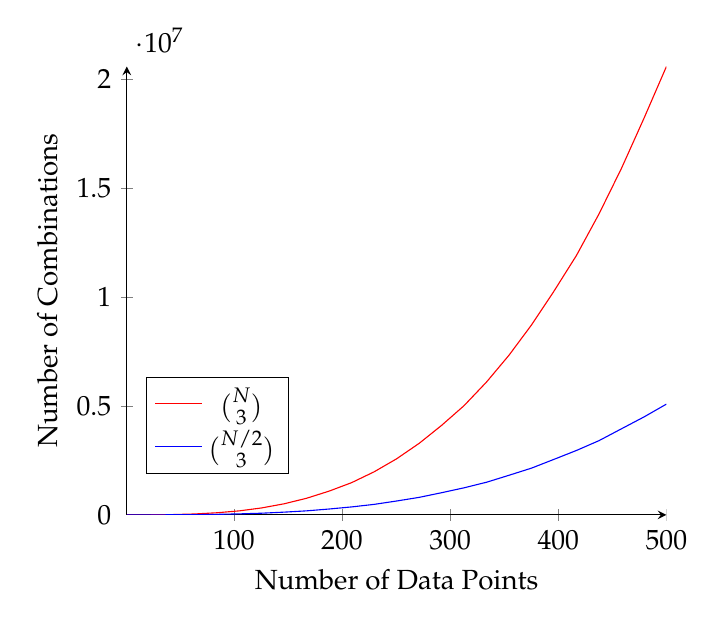
\begin{tikzpicture}
    \begin{axis} [
      axis lines = left,
      xlabel = Number of Data Points,
      ylabel = {Number of Combinations},
      legend style={at={(0.3,0.2)},anchor=east},
    ]
    \addplot [
    domain=1:500, 
    color=red,
    ]
    { factorial(x)/(factorial(x-3)*factorial(3))};
    \addplot [
    domain=1:500, 
    color=blue,
    ]
    { 2*factorial(x/2)/(factorial(x/2-3)*factorial(3)) };
        \addlegendentry{$\binom{N}{3}$}
    \addlegendentry{$\binom{N/2}{3}$}
    \end{axis}
  \end{tikzpicture}
  \caption{Number of combinations with $\binom{N}{3}$ compared to the number of combinations generated from $\binom{N/2}{3}$}
  \label{fig:binom_half_growth}
\end{figure}

The problem with this approach is the possible loss of information. Since the
algorithm has the threshold that defines how many entries a bin in the 
center histogram must have in order to be accepted as a radius/circle center.
This threshold should be high enough that triplets that contain noise points
do not contain to the circles but low enough that real circles with low point
can still be found.
\begin{figure}[tb]
   \centering
   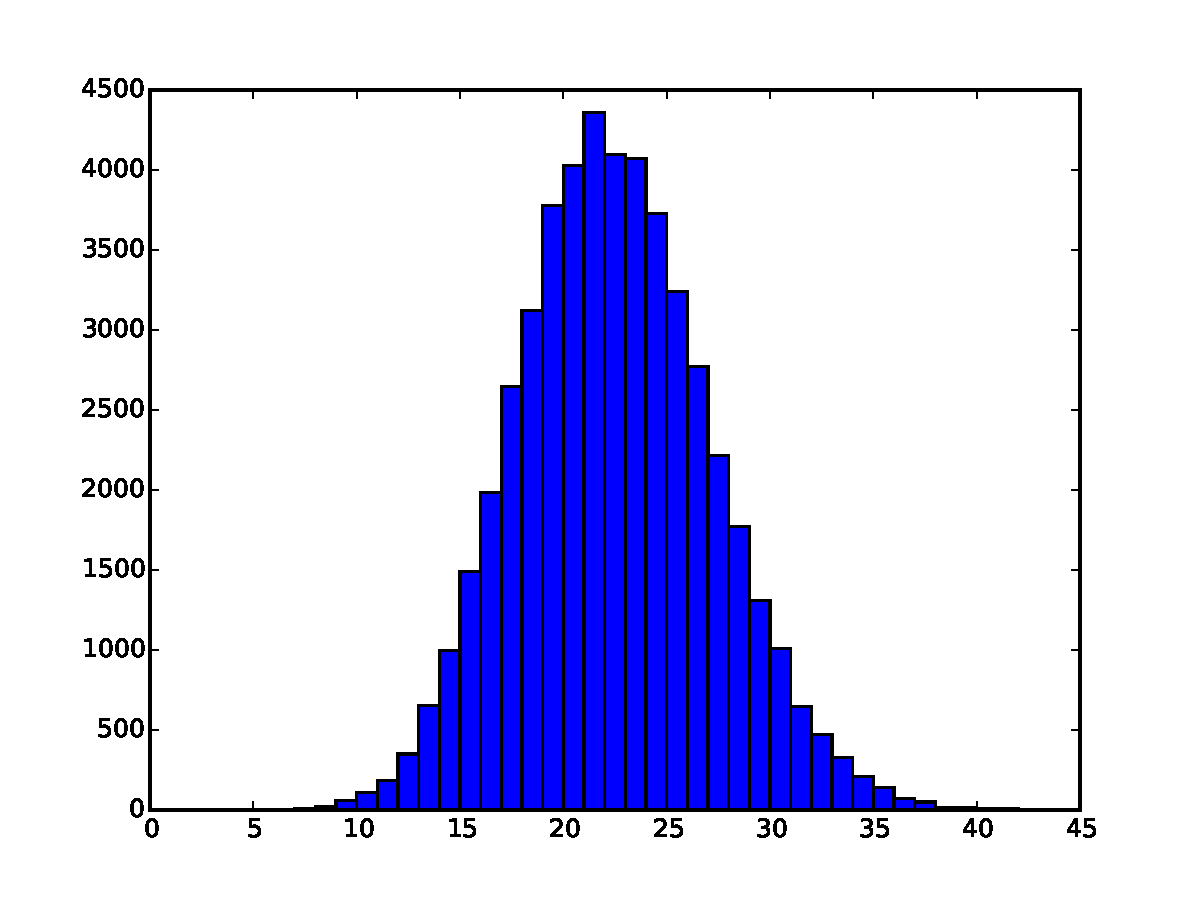
\includegraphics[width=0.8\textwidth]{pics/ppc}
   \caption{Distribution of points per circle. }
   \label{fig:ppc}
 \end{figure} 


If now the data is randomly split in two lists there are only 2 ways where
a circle with 10 hits will still be found namely that all the 10 points end
up in the same half of the list.
  \begin{table}[tb]
  \centering
  \caption{Example of ways to split points into 2 lists.}
    \label{tab:point_split}
  \begin{tabular}{cc}
  \toprule
  \textbf{Pts in list 1} & \textbf{Pts in list 2} \\
  \midrule
     10 & 0 \\
     9  & 1 \\
     8  & 2 \\
     $\vdots$ & $\vdots$ \\
     2 & 8\\
     1 & 9\\
     0 & 10 \\
  \bottomrule
  \end{tabular}

\end{table}

So the question is what are the probabilities that splitting a data set with
10 or more points ends up with 1 list having more than 10 points. As soon as
a circle has 20 points this becomes moot as always one list will have more 
than 10 points (see Figure~\ref{fig:ratios}).

From the figure it is clear that even if we split the lists there is a more 
than 50\% chance that we lose no information once a circle has 13 points.
\begin{figure}[htb]
  \centering
  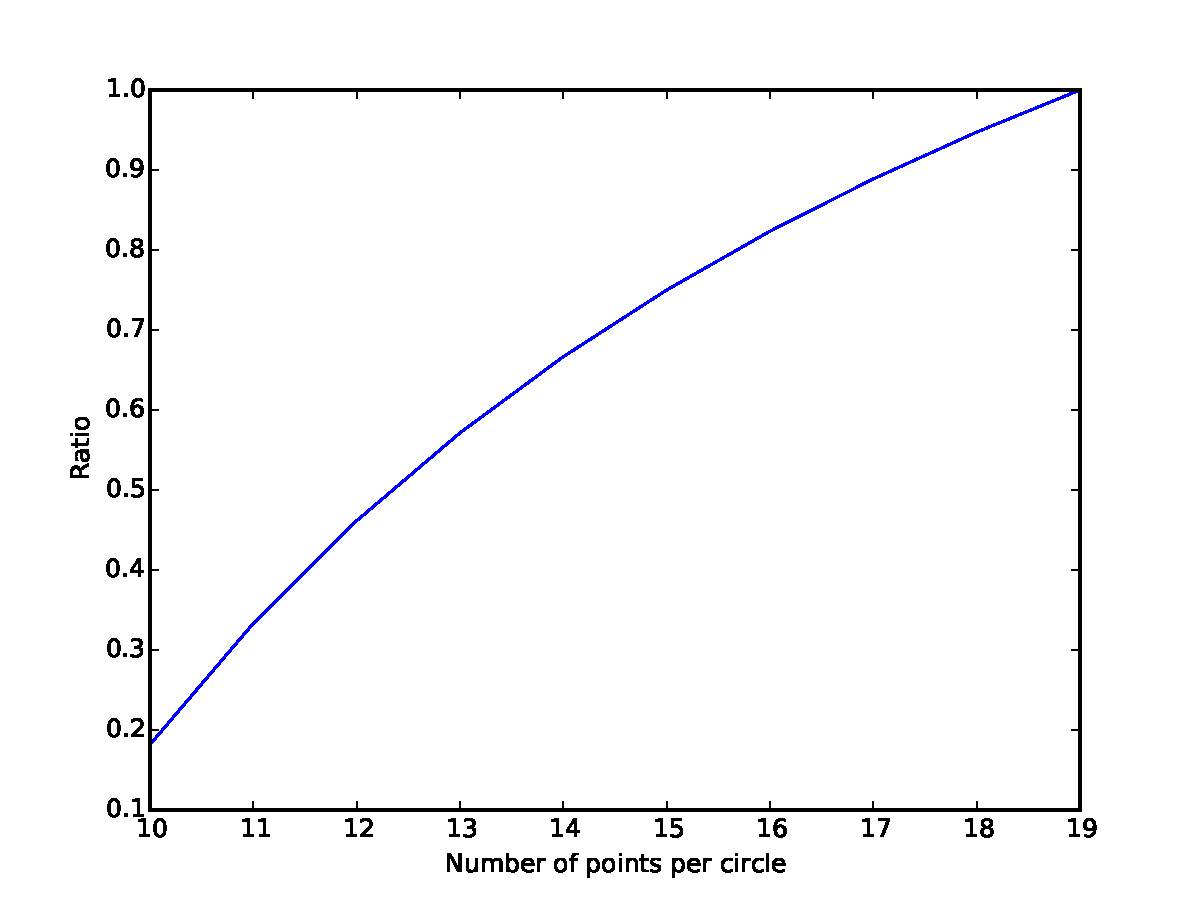
\includegraphics[width=\textwidth]{pics/ratio.pdf}
  \caption{The probability when splitting randomly a list of $x$ points into two that one list has more than 10 points.}
  \label{fig:ratios}
\end{figure}

% subsubsection optimisation (end)

\subsection{Possible Optimisation: Average Radius of Random Circles In a Unit Square} % (fold)
\label{ssub:average_radius_of_random_circles_in_a_unit_square}
An interesting property of calculating the radius of triplets generated from points that are distributed uniformely is that they always obey a certain shape.

First we calculate the expected area of a triangle formed by three points randomly chosen from the unit square\footnote{This prove is taken from \cite{Blatter:2015}}. Let \( A = (a_1, a_2),\ B = (b_1, b_2),\ C = (c_1, c_2)\) be the vertices of the random triangle \( T \). We consider the case where \( a_2
> b_2 > c_2 \) which takes $\frac{1}{6}$ of the total ``Volume''. Fix \( a_2, b_2, c_2 \) for the moment and we can write.
\[
  b_2 = (1-t)a_2 + tc_2, \qquad 0 \leq t \leq 1.
\]
The side $AC$ of $T$ intersects the horizontal level $y=b_2$ at the point $S=(s,b_2)$ with
\begin{equation}
  s = s(a_1,c_1,t) = (1-t)a_1 + tc_1
\end{equation}
The area $X$ of $T$ is then given by
\[
  X = \frac{1}{2}\lvert b_1 - s\rvert(c_2 - a_2)
\]
We now start integrating with respect to our six variables. The innermost integral is with respect to $b_1$ and gives

\begin{align}
  X_1 &:= \int_0^1X\text{d}b_1=\frac{1}{2}(c_2-a_2)\left( \int_0^s(s-b_1)db_1 + \int_s^1(b_1-s)db_1\right)\nonumber\\
      &\phantom{:}= \frac{1}{4}(c_2-a_2)(1+2s+2s^2)\nonumber
\end{align}
Next we integrate over $b_2$:
\begin{align}
  X_2 &:= \frac{1}{4}\int_0^1\int_{a_2}^1(c_2-a_2)^2\,dc_2\,da_2\,\times\,\int_0^1\int_0^1\int_0^1(1-2s+2s^2)\,dt\,dc_1\,da_1  \nonumber
\end{align}
This gives
\[
  X_3 = \frac{1}{4}\cdot \frac{1}{12} \cdot \frac{11}{18} = \frac{11}{6\cdot144}
\]
But generalizing our assumption at the beginning $a_2 < b_2 < c_2$ we multiply this result by $6$ and obtain then $\frac{11}{144}$.

% subsubsection average_radius_of_random_circles_in_a_unit_square (end)
% chapter methods (end)
\chapter{Results}
\label{cha:results}
In this section results for the conventional 1D, 2D, 3D Hough Transform and the combinatorial approach are presented. 1D and 2D Hough Transform
have no real application for the RICH detector since neither the center nor the radius is known. Nonetheless they are presented here as they offer a nice
way of understanding how each extra dimension expands the algorithm and also
shows the flaws with each added dimension.

For the 1D and 2D Hough Transform very simple data data was used. There were 
no physical constraints when generating the circles and their point/circle
or also their radius distribution doesn't reflect the real data obtained
by LHCb.

\section{1D Hough Transform Results} % (fold)
\label{sec:1d_hough_transform_results}
For this section different data sets were tested.
\begin{itemize}
  \item 1 circle and 600 background hits
  \item 2 circles and 0 background hits
  \item 5 circles and 30 background hits
\end{itemize}

For each set the radius score is shown and the final result of the algorithm.
The algorithm has no problems to find any of the circles even with background.
But this was expected as the algorithm only needs to search in one dimension
and makes the whole process very easy.

\subsection{Overview of the results} % (fold)
\label{sub:1d_overview_of_the_results}
First an overview about different test cases. The event with 1 circle and 600
background hits means to test how robust the algorithm is with a lot of
background hits. The second test case means to test if the algorithm can 
handle two circle objects and the third event is a mix between several
circles and some background hits.

There is are different plots
\begin{itemize}
  \item Radius score
  \item Resulting circle
\end{itemize}

The radius score is a 1D plot of the score function $f(r)$. The highest peak
indicating the maximum score and its location telling the value of the radius.
The resulting circle plot is the center (which was known) and the extracted radius combined, drawing the resulting circle. There is always the same plot
again with center and radius taken directly from data to compare the two results.

% subsection overview_of_the_results (end)
\begin{figure}[htp]
        \centering
        \begin{subfigure}[t]{0.3\textwidth}
                \centering
                \includegraphics[width=\textwidth]{sim_pics/1D_HT/result_1_circle_600_bg}
                \caption{1 circle, 600 background hits.}
                \label{fig:1c600bg}
        \end{subfigure}%
        ~ %add desired spacing between images, e. g. ~, \quad, \qquad etc.
          %(or a blank line to force the subfigure onto a new line)
        \begin{subfigure}[t]{0.3\textwidth}
                \centering
                \includegraphics[width=\textwidth]{sim_pics/1D_HT/result_2_circles_0_bg}
                \caption{2 circles, 0 background hits}
                \label{fig:2c0bg}
        \end{subfigure}%
        ~ %add desired spacing between images, e. g. ~, \quad, \qquad etc.
          %(or a blank line to force the subfigure onto a new line)
        \begin{subfigure}[t]{0.3\textwidth}
                \centering
                \includegraphics[width=\textwidth]{sim_pics/1D_HT/result_5_circles_30_bg}
                \caption{5 circles, 30 background hits}
                \label{fig:5c30bg}
        \end{subfigure}
        \caption{Circles found by the 1D Hough Transform. The circle in Figure~\ref{fig:1c600bg} has its center in the origin so the algorithm did find the circle.}\label{fig:1d_ht_results}

                \begin{subfigure}[t]{0.3\textwidth}
                \centering
                \includegraphics[width=\textwidth]{sim_pics/1D_HT/real_result_1_circle_600_bg}
                \caption{1 circle, 600 background hits.}
                \label{fig:real_1c600bg}
        \end{subfigure}%
        ~ %add desired spacing between images, e. g. ~, \quad, \qquad etc.
          %(or a blank line to force the subfigure onto a new line)
        \begin{subfigure}[t]{0.3\textwidth}
                \centering
                \includegraphics[width=\textwidth]{sim_pics/1D_HT/real_result_2_circles_0_bg}
                \caption{2 circles, 0 background hits}
                \label{fig:real_2c0bg}
        \end{subfigure}%
        ~ %add desired spacing between images, e. g. ~, \quad, \qquad etc.
          %(or a blank line to force the subfigure onto a new line)
        \begin{subfigure}[t]{0.3\textwidth}
                \centering
                \includegraphics[width=\textwidth]{sim_pics/1D_HT/real_result_5_circles_30_bg}
                \caption{5 circles, 30 background hits}
                \label{fig:real_5c30bg}
        \end{subfigure}
        \caption{These are the circles as generated by the simulation. All of these examples were correctly solved by the 1D Hough Transform.}\label{fig:real_1d_ht_results}
\end{figure}

\subsection{1D Hough Transform - 2 circles, 0 background} % (fold)
\label{sub:1d_hough_transform_2_circles_0_background}
Two circle objects have to be found in this event with zero background.
% subsection 1d_hough_transform_2_circles_0_background (end)
\begin{figure}[htp]
        \centering
        \begin{subfigure}[t]{0.5\textwidth}
                \centering
                \includegraphics[width=\textwidth]{pics/1D_HT/radius_scores_2_circles_0_bg_1}
                \caption{1 circle, 600 background hits.}
                \label{fig:2c0bg_radius1}
        \end{subfigure}%
        \begin{subfigure}[t]{0.5\textwidth}
                \centering
                \includegraphics[width=\textwidth]{pics/1D_HT/radius_scores_2_circles_0_bg_2}
                \caption{2 circles, 0 background hits}
                \label{fig:2c0b_radius2}
        \end{subfigure}
        \caption{Radius score for the 1D Hough Transform for 2 circles with 0 background. The respective radiuses are $0.191$ and $0.108$ }\label{fig:1d_ht_radius}
\end{figure}
Each peaks is clearly visible in their respective radius score plots. The algorithm has no problems finding two distinct circles in the plane. A problem
would then occur if
\clearpage
\subsection{1D Hough Transform - 5 circles, 30 background hits} % (fold)
\label{sub:1d_hough_transform_5_circles_30_background_hits}
First we have the different radius scores for each known center. So the algorithm calculates the score for one center with all data points at a
time and the radius with the highest score gets assigned to that center.
Once done for all centers the algorithm is done.
\begin{figure}[htbp]
  \centering
  \begin{subfigure}{0.3\textwidth}
  \centering
  \includegraphics[width=\textwidth]{sim_pics/1D_HT/radius_scores_5_circles_30_bg_1}
  \end{subfigure}
  \begin{subfigure}{0.3\textwidth}
  \centering
  \includegraphics[width=\textwidth]{sim_pics/1D_HT/radius_scores_5_circles_30_bg_2}
  \end{subfigure}
      \begin{subfigure}{0.3\textwidth}
  \centering
  \includegraphics[width=\textwidth]{sim_pics/1D_HT/radius_scores_5_circles_30_bg_3}
  \end{subfigure}

  \begin{subfigure}{0.3\textwidth}
  \centering
  \includegraphics[width=\textwidth]{sim_pics/1D_HT/radius_scores_5_circles_30_bg_4}
  \end{subfigure}
  \begin{subfigure}{0.3\textwidth}
  \centering
  \includegraphics[width=\textwidth]{sim_pics/1D_HT/radius_scores_5_circles_30_bg_5}
  \end{subfigure}
  \caption{Radius scores for all the centers for an event with 5 circles.}
  \label{fig:5_circles_30_bg_radius}
\end{figure}
As exptected the circles can be reconstructed
\begin{figure}[htbp]
  \centering
  \begin{subfigure}{0.45\textwidth}
  \includegraphics[width=\textwidth]{sim_pics/1D_HT/result_5_circles_30_bg}
  \end{subfigure}
  \begin{subfigure}{0.45\textwidth}
  \includegraphics[width=\textwidth]{sim_pics/1D_HT/real_result_5_circles_30_bg}
  \end{subfigure}
  \caption{The reconstructed result on the left while the circles from the simulated data is on the right.}
  \label{fig:figure1}
\end{figure}
% subsection 1d_hough_transform_5_circles_30_background_hits (end)


% section 1d_hough_transform_results (end)

\clearpage
\section{2D Hough Transform Results} % (fold)
\label{sec:2d_hough_transform_results}
The 2D Hough Transform searches in the $x,y$ space for suitable
circle centers that have a high score. The same events as for the 1D
Hough Transform were investigated to make a comparison about reliability.
In a first overview the algorithm performs quite well and finds all the
circles.

Again among others there were some of the events tackled by the algorithm.
\begin{itemize}
  \item 1 circle and 600 background hits
  \item 2 circles and 0 background hits
  \item 5 circles and 30 background hits
\end{itemize} 

\subsection{Overview of the results} % (fold)
\label{sub:2d_overview_of_the_results}
As in subsection \ref{sub:1d_overview_of_the_results} in a first step an overview of the results. The same events as before but this time tested with the 2D
Hough Transform. All the circles were found correctly but the example with 6 circles and 200 background hits shows that the algorithm can fail to find a 
circle.
% subsection overview_of_the_results (end)

\begin{figure}[htp]
        \centering
        \begin{subfigure}[t]{0.3\textwidth}
                \centering
                \includegraphics[width=\textwidth]{sim_pics/2D_HT/result_1_circle_600_bg}
                \caption{1 circle, 600 background hits. The circle is centered at $0.0/0.0$.}
                \label{fig:2d_1c600bg}
        \end{subfigure}%
        ~ %add desired spacing between images, e. g. ~, \quad, \qquad etc.
          %(or a blank line to force the subfigure onto a new line)
        \begin{subfigure}[t]{0.3\textwidth}
                \centering
                \includegraphics[width=\textwidth]{sim_pics/2D_HT/result_2_circles_0_bg}
                \caption{2 circles, 0 background hits}
                \label{fig:2d_2c0bg}
        \end{subfigure}%
        ~ %add desired spacing between images, e. g. ~, \quad, \qquad etc.
          %(or a blank line to force the subfigure onto a new line)
        \begin{subfigure}[t]{0.3\textwidth}
                \centering
                \includegraphics[width=\textwidth]{sim_pics/2D_HT/result_5_circles_30_bg}
                \caption{5 circles, 30 background hits}
                \label{fig:2d_5c30bg}
        \end{subfigure}
        \caption{Circles found by the 2D Hough Transform. The circle in Figure~\ref{fig:1c600bg} has its center in the origin so the algorithm did find the circle.}\label{fig:2D_HT_results}

                \begin{subfigure}[t]{0.3\textwidth}
                \centering
                \includegraphics[width=\textwidth]{sim_pics/2D_HT/real_result_1_circle_600_bg}
                \caption{1 circle, 600 background hits.}
                \label{fig:2d_real_1c600bg}
        \end{subfigure}%
        ~ %add desired spacing between images, e. g. ~, \quad, \qquad etc.
          %(or a blank line to force the subfigure onto a new line)
        \begin{subfigure}[t]{0.3\textwidth}
                \centering
                \includegraphics[width=\textwidth]{sim_pics/2D_HT/real_result_2_circles_0_bg}
                \caption{2 circles, 0 background hits}
                \label{fig:2d_real_2c0bg}
        \end{subfigure}%
        ~ %add desired spacing between images, e. g. ~, \quad, \qquad etc.
          %(or a blank line to force the subfigure onto a new line)
        \begin{subfigure}[t]{0.3\textwidth}
                \centering
                \includegraphics[width=\textwidth]{sim_pics/2D_HT/real_result_5_circles_30_bg}
                \caption{5 circles, 30 background hits}
                \label{fig:2d_real_5c30bg}
        \end{subfigure}
        \caption{These are the circles as generated by the simulation. All of these examples were correctly solved by the 2D Hough Transform.}\label{fig:real_2d_ht_results}

        \begin{subfigure}{0.47\textwidth}
          \centering
          \includegraphics[width=\textwidth]{sim_pics/2D_HT/result_6_circles_200_bg}
        \end{subfigure}
        \begin{subfigure}{0.47\textwidth}
          \centering
          \includegraphics[width=\textwidth]{sim_pics/2D_HT/real_result_6_circles_200_bg}
        \end{subfigure}
        \caption{Circles found by the algorithm on the left and the correct results on the right. Here the 2D Hough Transform fails to find the magenta colored circle.}
        \label{fig:2d_6c_200_bg}
\end{figure}
As seen in the event with 6 circles and 200 background hits (Figure~\ref{fig:2d_6c_200_bg}), the 2D Hough Transform fails. The reason is quite simple. Both, the yellow and magenta circle, have similar radiuses. Now the algorithm looks first for the magenta circle (because that happens to be the way the centers are arranged in the list) and since so many points of the yellow circle lie so close together it is easy for the magenta circle (who has a similar radius) to get a high score with these points, a higher score than it would get with its proper points. If the yellow points were more evenly distributed on the circle or if there were more magenta points this probably wouldn't happen but that is something that can't be controlled.

Theoretically it is also possible that the yellow circle gets fitted to the
magenta points but since there are still enough yellow points left after the removal of the points assigned to the magenta circle they still have the highest score with their own points and the magenta circle goes unnoticed.

Also, if the yellow circle would be checked before magenta then the algorithm
would find the proper circles as well. So it actually can depend on the order
in which the circles are searched.

\subsection{2D Hough Transform, 2 circles, 0 background hits} % (fold)
\label{sub:2d_hough_transform_2_circles_0_background}
Two circle objects have to be found in this event with zero background. This
poses no problem but as pointed out before if the two circles had a 
\begin{figure}[htp]
        \centering
        \begin{subfigure}[t]{0.5\textwidth}
                \centering
                \includegraphics[width=\textwidth]{sim_pics/2D_HT/center_scores_2_circles_0_bg_1}
        \end{subfigure}%
        \begin{subfigure}[t]{0.5\textwidth}
                \centering
                \includegraphics[width=\textwidth]{sim_pics/2D_HT/center_scores_2_circles_0_bg_2}
        \end{subfigure}
        \caption{Center score for the 2D Hough Transform for 2 circles with 0 background.}\label{fig:2d_ht_center}
x
        \begin{subfigure}[t]{0.5\textwidth}
                \centering
                \includegraphics[width=\textwidth]{sim_pics/2D_HT/result_2_circles_0_bg}
        \end{subfigure}%
        \begin{subfigure}[t]{0.5\textwidth}
                \centering
                \includegraphics[width=\textwidth]{sim_pics/2D_HT/real_result_2_circles_0_bg}
        \end{subfigure}
\caption{Although already shown before for completeness the 2 circle 2D Hough Transform result. Left side the result from the algorithm on the right side the correct result from data.}
\end{figure}

% subsection 2d_hough_transform_2_circles_0_background (end)

\clearpage
\subsection{2D Hough Transform, 5 circles, 30 background hits} % (fold)
\label{sub:2d_hough_transform_5_circles_30_background_hits}

This event added more circles but also some background hits. Both were handled
well by the algorithm and all the circles were found.

\begin{figure}[htbp]
  \centering
  \begin{subfigure}{0.32\textwidth}
  \centering
  \includegraphics[width=\textwidth]{sim_pics/2D_HT/center_scores_5_circles_30_bg_1}
  \end{subfigure}
  \begin{subfigure}{0.32\textwidth}
  \centering
  \includegraphics[width=\textwidth]{sim_pics/2D_HT/center_scores_5_circles_30_bg_2}
  \end{subfigure}
  \begin{subfigure}{0.32\textwidth}
  \centering
  \includegraphics[width=\textwidth]{sim_pics/2D_HT/center_scores_5_circles_30_bg_3}
  \end{subfigure}
  
  \begin{subfigure}{0.32\textwidth}
  \centering
  \includegraphics[width=\textwidth]{sim_pics/2D_HT/center_scores_5_circles_30_bg_4}
  \end{subfigure}
  \begin{subfigure}{0.32\textwidth}
  \centering
  \includegraphics[width=\textwidth]{sim_pics/2D_HT/center_scores_5_circles_30_bg_5}
  \end{subfigure}
  \caption{Center scores for all the centers for an event with 5 circles.}
  \label{fig:2d_5_circles_30_bg_radius}
\end{figure}
\begin{figure}[htbp]
  \centering
  \begin{subfigure}{0.45\textwidth}
  \includegraphics[width=\textwidth]{sim_pics/2D_HT/result_5_circles_30_bg}
  \end{subfigure}
  \begin{subfigure}{0.45\textwidth}
  \includegraphics[width=\textwidth]{sim_pics/2D_HT/real_result_5_circles_30_bg}
  \end{subfigure}
  \caption{The reconstructed result on the left while the circles from the simulated data is on the right.}
  \label{fig:2d_5c_results}
\end{figure}
% subsection 2d_hough_transform_5_circles_30_background_hits (end)

\subsection{2D Hough Transform, 6 circles, 200 background hits} % (fold)
\label{sub:2d_hough_transform_6_circles_200_background_hits}
As briefly discussed in the overview the algorithm does make mistakes as seen
in this next event. 6 circles were generated with 200 background hits. The
interesting part is not that amount of circles or the amount of background hits
posed a problem but the properties of the circles (center coordinate and radius). In this example there is a misidentification of a circle with points
of another.
% subsection 2d_hough_transform_6_circles_200_background_hits (end)

\begin{figure}
\centering
  \begin{subfigure}{0.3\textwidth}
  \centering
    \includegraphics[width=\textwidth]{sim_pics/2D_HT/center_scores_6_circles_200_bg_1}
  \end{subfigure}
  \begin{subfigure}{0.3\textwidth}
    \centering
    \includegraphics[width=\textwidth]{sim_pics/2D_HT/center_scores_6_circles_200_bg_2}
  \end{subfigure}
  \begin{subfigure}{0.3\textwidth}
  \centering
    \includegraphics[width=\textwidth]{sim_pics/2D_HT/center_scores_6_circles_200_bg_3}
  \end{subfigure}

  \begin{subfigure}{0.3\textwidth}
  \centering
    \includegraphics[width=\textwidth]{sim_pics/2D_HT/center_scores_6_circles_200_bg_4}
  \end{subfigure}
  \begin{subfigure}{0.3\textwidth}
  \centering
    \includegraphics[width=\textwidth]{sim_pics/2D_HT/center_scores_6_circles_200_bg_5}
  \end{subfigure}
  \begin{subfigure}{0.3\textwidth}
  \centering
    \includegraphics[width=\textwidth]{sim_pics/2D_HT/center_scores_6_circles_200_bg_6}
  \end{subfigure}
  \caption{Center scores for 6 circles with 200 background hits. There is a lot more going on because of all the background hits that by accident contribute to a high score all over the grid.}
\end{figure}
\begin{figure}
\begin{subfigure}{0.5\textwidth}
  \includegraphics[width=\textwidth]{sim_pics/2D_HT/result_6_circles_200_bg}
\end{subfigure}
\begin{subfigure}{0.5\textwidth}
  \includegraphics[width=\textwidth]{sim_pics/2D_HT/real_result_6_circles_200_bg}
\end{subfigure}
\caption{On the left side the wrong result obtained by the 2D Hough Transform and the correct one on the right side}
\end{figure}

A possible way to fix this particular problem is to tune the parameters of the weight function namely reducing the standard deviation. 
\[
  w(\eta) = \frac{1}{\sqrt{2\pi}\sigma}\exp\left( \frac{-\eta^2}{2\sigma^2}\right)
\]
Having a higher $\sigma$ means that a point that is a bit off of the circle still contributes a considerable value to the total score. The smaller the $\sigma$ is the sharper the peak. However if the peak is too sharp then the algorithm might discard possible results because they are just a bit off the circle but since the peak is so narrow they don't contribute at all to the total score.

In the example before $\sigma$ was equal to $0.001$ while the space dimension was $1$. So if the detector was $1$\,m per dimension a hit $1$\,mm off the perfect location contributes still more half of the score off the perfect location. If we set $\sigma=0.0005$ a point $0.001$ away from the perfect location it only contributes about $14\%$ of the maximum score.

\begin{figure}
\centering
  \begin{subfigure}{.49\textwidth}

    \includegraphics[width=\textwidth]{sim_pics/2D_HT/center_scores_6_circles_200_bg_5}
  \end{subfigure}
  \begin{subfigure}{.49\textwidth}

    \includegraphics[width=\textwidth]{sim_pics/2D_HT/center_scores_6_circles_200_bg_6}
  \end{subfigure}

  \begin{subfigure}{.49\textwidth}

    \includegraphics[width=\textwidth]{sim_pics/2D_HT/center_scores_6_circles_200_bg_5_corr}
  \end{subfigure}
  \begin{subfigure}{.49\textwidth}

    \includegraphics[width=\textwidth]{sim_pics/2D_HT/center_scores_6_circles_200_bg_6_corr}
  \end{subfigure}
  \caption{Old center score in the top row for circle 5 (magenta) and 6 (yellow). And below the same circles this time with the new $\sigma=0.0005$. Something that quite clear is how big the influence of sigma is for the center score. With a $\sigma$ of $0.001$ just by eye there seem to be many similar maxima whereas with a $\sigma=0.0005$ the maximas get much more distinct.}
\end{figure}

\begin{figure}
\centering
\begin{subfigure}{0.49\textwidth}
  \includegraphics[width=\textwidth]{sim_pics/2D_HT/result_6_circles_200_bg_corr}
\end{subfigure}
\begin{subfigure}{0.49\textwidth}
  \includegraphics[width=\textwidth]{sim_pics/2D_HT/real_result_6_circles_200_bg}
\end{subfigure}
\caption{Again on the left the calculated result and the result taken from data on the right. With the new $\sigma$ the algorithm is able to calculate all the circles correctly.}\label{2d_result_6c_200bg_corr}
\end{figure}

% section 2d_hough_transform_results (end)

\section{3D Hough Transform Results} % (fold)
\label{sec:3d_hough_transform_results}

% section 3d_hough_transform_results (end)

\section{Combinatorial Approach Results} % (fold)
\label{sec:combinatorial_approach_results}

% section combinatorial_approach_results (end)
% chapter results (end)

\chapter{Conclusions} % (fold)
\label{cha:conclusions}

This thesis was studying different Hough Transforms for circle detection. In a first approach a 1D Hough Transform was used and then extended to two and three
dimensions.
As a fourth and final approach a new method was developped for the circle detection. 

% chapter conclusions (end)

\printbibliography
\end{document}
